\documentclass[slide,papersize]{jsarticle}
\usepackage[dvipdfmx]{graphicx,color}
\begin{document}

\section*{HelloWorld}
\vspace*{15mm}
\begin{center}
{\Huge {\bf Hello World}}
\end{center}

\section*{Hello World}
\bigskip
\begin{itemize}
\item 作ってみよう、動かしてみよう
\bigskip
\item Android Manifest
\bigskip
\item DDMS
\bigskip
\item Log
\end{itemize}

\section*{作ってみよう}
\bigskip
\begin{itemize}
\item File → New → Project → Android Project
\end{itemize}

\section*{動かしてみよう}
\bigskip
\begin{itemize}
\item まずはエミュレータで起動
\bigskip
\item 方法は略
\end{itemize}

\section*{やってみよう}
\bigskip
\begin{itemize}
\item Project Name : HelloAndroid
\medskip
\item Build Target : Google APIs 1.6
\medskip
\item Application name : Hello
\medskip
\item Package name : com.example.hello.android
\medskip
\item Create Activity : HelloActivity
\end{itemize}

\section*{実機デバッグの方法}
\bigskip
\begin{itemize}
\item 実機の設定
 \begin{itemize}
 \item {\footnotesize 設定→アプリケーション→開発→USBデバッグ}
 \end{itemize}
\bigskip
\item マニフェストの修正
 \begin{itemize}
 \item {\footnotesize Application タブの Debuggable を true に}
 \item {\footnotesize これはデバッグする時に必要}
 \end{itemize}
\end{itemize}
後は (ほぼ) 一緒です

\section*{実機デバッグの設定}
\medskip
Ubuntu の例です
\begin{itemize}
\item /etc/udev/rules.d/51-android.rules の作成\\
{\tiny \begin{verbatim}SUBSYSTEM=="usb", SYSFS{idVendor}=="0bb4", MODE="0666"\end{verbatim}}
%% \begin{itemize}
%% \item 中身は以下
%% \item {\tiny \begin{verbatim}SUBSYSTEM=="usb", SYSFS{idVendor}=="0bb4", MODE="0666"\end{verbatim}}
%% \end{itemize}
\item 権限の付与\\
{\tiny \begin{verbatim}# chmod a+r /etc/udev/rules.d/51-android.rules\end{verbatim}}
%% \begin{itemize}
%% \item {\tiny \begin{verbatim}# chmod a+r /etc/udev/rules.d/51-android.rules\end{verbatim}}
%% \end{itemize}
\bigskip
\item http://bit.ly/aH647W
\end{itemize}

\section*{できれば}
\vspace*{17mm}
\begin{center}
{\Huge {\bf 実機でも}}
\end{center}

\section*{Android Manifest}
\bigskip
\begin{itemize}
\item permission
\bigskip
\item サービス
\bigskip
\item コンテントプロバイダ
\bigskip
\item Activity
\end{itemize}

\section*{DDMS}
\bigskip
\begin{itemize}
\item Device
\bigskip
\item Emulator Control
\bigskip
\item LogCat
\bigskip
\item File Explore
\end{itemize}

\section*{Log 抽出}
\bigskip
\begin{itemize}
\item ログレベルについて
\bigskip
\item 抽出の方法
\bigskip
\item export
\end{itemize}

\section*{Log 出力について}
\bigskip
\begin{itemize}
\item ハロワに盛り込んでみる
 \begin{itemize}
 \item 例) Log.d(``tag'', ``message'');
 \medskip
 \item onCreate() 内にて出力させてみる
 \end{itemize}
\bigskip
\item Log 出力確認など
\end{itemize}

\section*{やってみよう}
\bigskip
\begin{itemize}
\item エミュレータで試してみる
\bigskip
\item 実機で試してみる
\end{itemize}

\section*{例外発生時}
{\footnotesize 以下な状態になった場合ログを確認してみましょう}
\begin{center}
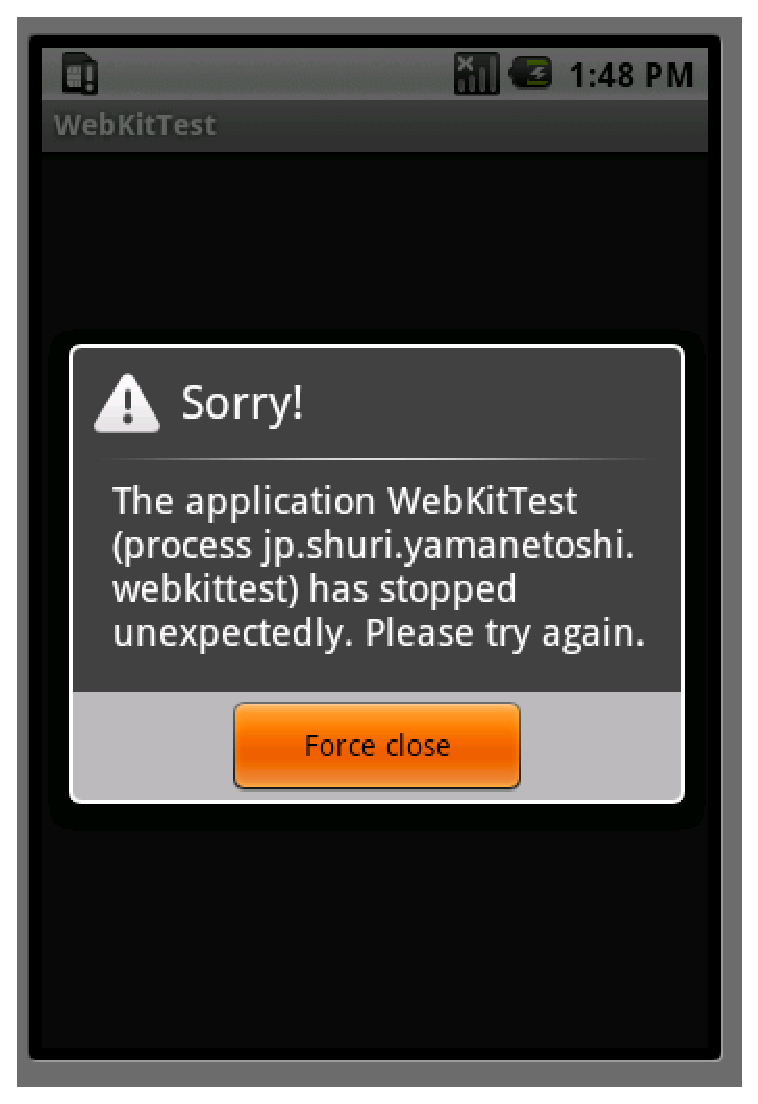
\includegraphics[scale=0.18]{nulpoexp.eps}
\end{center}

\section*{当該ログ}
\begin{center}
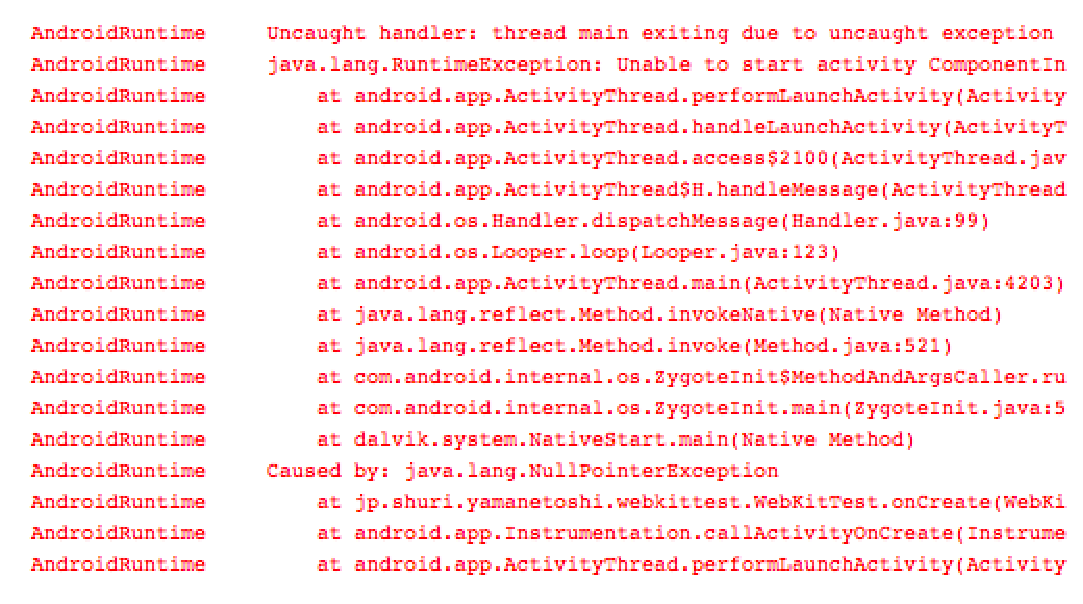
\includegraphics[scale=0.3]{nulpoLog.eps}
\end{center}
こんなカンジで例外メセジが見れます

\end{document}
